\justifying
Para activar la paginacion es necesario que armemos el sistema de directorios y paginas del kernel. Como se requirio un identity mapping para el kernel, de los primeros 7.5Mb de memoria, utilizamos entradas en el directorio. La primer entrada posee todas las posiciones de la tabla inicializadas en Present, marcando asi los primeros 4Mb. La segunda entrada, sin embargo solo debe mapear 3.5Mb, con lo cual solo se necesitan 896 entradas mas marcadas como presentes.\\

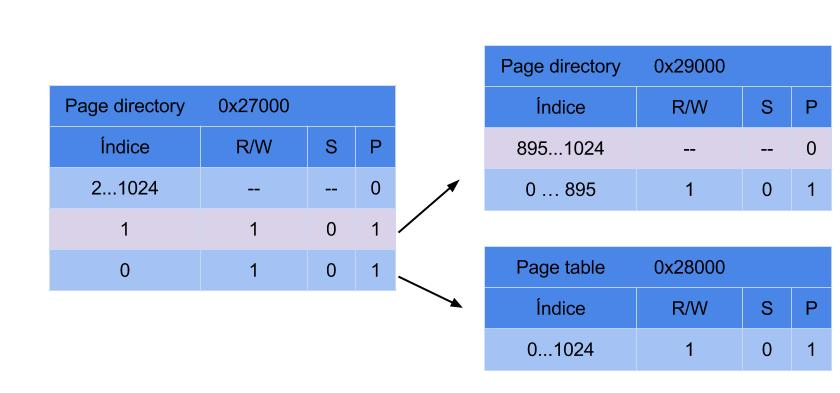
\includegraphics[scale=0.4]{diagramas/paginacionKernel.jpg}
\\\centering{Distribucion de paginas del kernel y posicion de los directorios.}\\
\justifying
Para el paginado de las tareas se requerian por enunciado 3 paginas: 2 para la tarea que debian mapearse en el mar (arriba del primer giga) y una tercera, el ancla, que debia apuntar al espacio de memoria del kernel (no modificable). La estructura del directorio y de las tablas se pusieron contiguas a las del kernel, en su area de memoria. Para ubicar las tareas a partir de la direccion virtual 0x40000000, se utilizo el indice 256 de sus directorios y cada tabla apuntando de a 4Mb: 0x40000000, 40001000 y 40002000. Tambien fue necesario inicializar 2 entradas en el directorio de cada tarea con identity mapping a la memoria del kernel, para que este pudiese ejecutarse en el contexto de la tarea. Estas entradas poseen acceso solo por el kernel y permiten la ejecucion de los handlers de interrupciones.

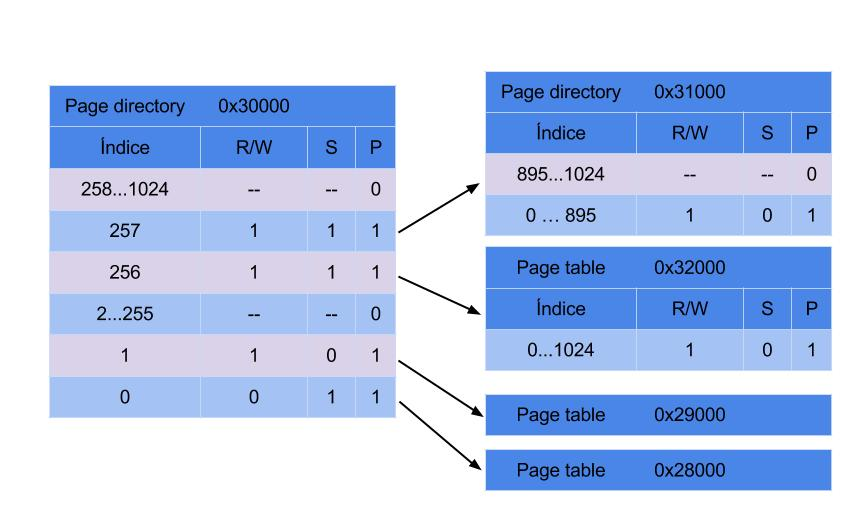
\includegraphics[scale=0.4]{diagramas/paginacionTarea.jpg}
\\\centering{Mapeo generico de una tarea.}\\
\justifying
Como las tareas son capaces de "moverse" se puso a disposicion de la mmu funciones para remapear las paginas propias. Se paso de forma mas directa la informacion soblre las paginas al Context Manager para poder reflejar el movimiento de las paginas en la pantalla del mapa y en los indicadores de la pantalla de estado. 

